\documentclass{article}
\usepackage[utf8]{inputenc}
\usepackage[a4paper,textwidth=6in,top=20mm,bottom=25mm]{geometry}
\usepackage{graphicx}
\usepackage{parskip}
\usepackage{amsmath,amsfonts,amsthm}
\usepackage{hyperref}
\usepackage[section]{placeins}
\usepackage[backend=bibtex]{biblatex}
\addbibresource{ref.bib}
\hypersetup{colorlinks=true,linkcolor=blue,urlcolor=blue}
\urlstyle{same}
\newtheorem{proposition}{Proposition}
\title{Async Swap: Coincidence-of-Wants Matching on Uniswap v4}
\author{Msaki, Meek \and Li, Jiasun}
\date{October 23, 2026}

\begin{document}
\maketitle

\begin{abstract}
Async Swap is an on-chain limit-order protocol that separates the commitment to trade from
execution. Makers escrow an input amount and specify a minimum output. Compatible orders
exchange their escrows directly; unmatched amounts remain available to later counterparties,
pool liquidity, or independent fillers. USDC provides a common unit of account. Price buckets
organize the book, while exact rational limits determine which orders can trade. Escrowed
priority bids rank eligible orders within each bucket. Subtree price summaries locate the
highest-priority eligible order without scanning incompatible orders. We characterize feasible
transfers, give integer settlement rules that preserve both makers' limits, and derive bounds
on matching work. The design trades immediate execution for price control while keeping
settlement atomic and the book's work per matching call bounded.
\end{abstract}

\section{The problem: price control and execution cost}

Immediate execution consumes the liquidity available at the time of a trade. In a constant-product
pool with asset reserve $X$ and quote reserve $Y$, selling $z$ asset units yields, before fees,
\begin{equation}
 Q(z)=\frac{Yz}{X+z},\qquad
 \frac{Q(z)}{z}=\frac{Y}{X+z},\qquad
 \frac{d}{dz}\frac{Q(z)}{z}=-\frac{Y}{(X+z)^2}.
\end{equation}
The average execution price declines as trade size grows relative to available liquidity.
Concentrated liquidity changes the depth available over each price range, but execution
still depends on that depth~\cite{UniswapV3}. A maker willing to wait can instead state a
limit and exchange with a compatible counterparty. Direct matching avoids consuming pool
liquidity for the matched portion; it does not ensure that a counterparty will arrive.

An on-chain book must reconcile three requirements: respect exact limits, assign an explicit
priority among competing orders, and bound the work needed to find a match. Grouping nearby
prices makes indexing practical, but a high-priority order in a group may be incompatible
with a counterparty that can trade with another order in the same group. Async Swap separates
\emph{price grouping}, \emph{eligibility}, and \emph{priority} so that grouping cannot create
this obstruction.

\section{Orders and feasible exchange}

Each market pairs an asset with USDC. An order specifies its owner, side, remaining input,
minimum output for that input, escrowed priority bid, and arrival sequence. The input and bid
are reserved when the order is admitted. Minimum outputs are positive. A limit applies
proportionally to each partial fill; any unspent input remains reserved or is returned to
the maker when the order closes.

Let a seller offer $S>0$ asset units for at least $Q_s>0$ USDC units. Let a buyer offer
$B>0$ USDC units for at least $A_b>0$ asset units. Amounts are measured in integer token
base units unless stated otherwise. Their exact limits, in USDC base units per asset base
unit, are
\begin{equation}
 p_s=\frac{Q_s}{S},\qquad p_b=\frac{B}{A_b}.
\end{equation}
A transfer of $x$ asset units and $q$ USDC units is feasible when
\begin{equation}
 \mathcal F=\{(x,q):0<x\le S,\;0<q\le B,\;p_sx\le q\le p_bx\}.
 \label{eq:feasible}
\end{equation}
Ignoring indivisibility for the moment, $\mathcal F$ is nonempty exactly when
\begin{equation}
 p_s\le p_b\quad\Longleftrightarrow\quad Q_sA_b\le BS.
 \label{eq:cross}
\end{equation}
At an execution price $p\in[p_s,p_b]$, the largest continuous transfer at that price is
\begin{equation}
 x(p)=\min\{S,B/p\},\qquad q(p)=p\,x(p).
 \label{eq:frontier}
\end{equation}
Thus the maximum asset transfer is $\min\{S,B/p_s\}$, attained at the seller's limit;
the maximum USDC transfer is $\min\{B,Sp_b\}$, attained at the buyer's limit. These are
pairwise bounds, not a claim that one allocation maximizes welfare or future trading volume.

For example, using whole-token units, take $S=2$, $Q_s=2000$, $B=1650$, and $A_b=1.5$.
The acceptable interval is $[1000,1100]$ USDC per asset. At the seller's limit the pair
exchanges $1.65$ assets for $1650$ USDC; at the buyer's limit it exchanges $1.5$ assets for
the same USDC amount. The intersections of the two limit lines with $q=B$ determine these
quantities. Priority fees are separate from the exchange amounts.

\begin{figure}[htbp]
\centering
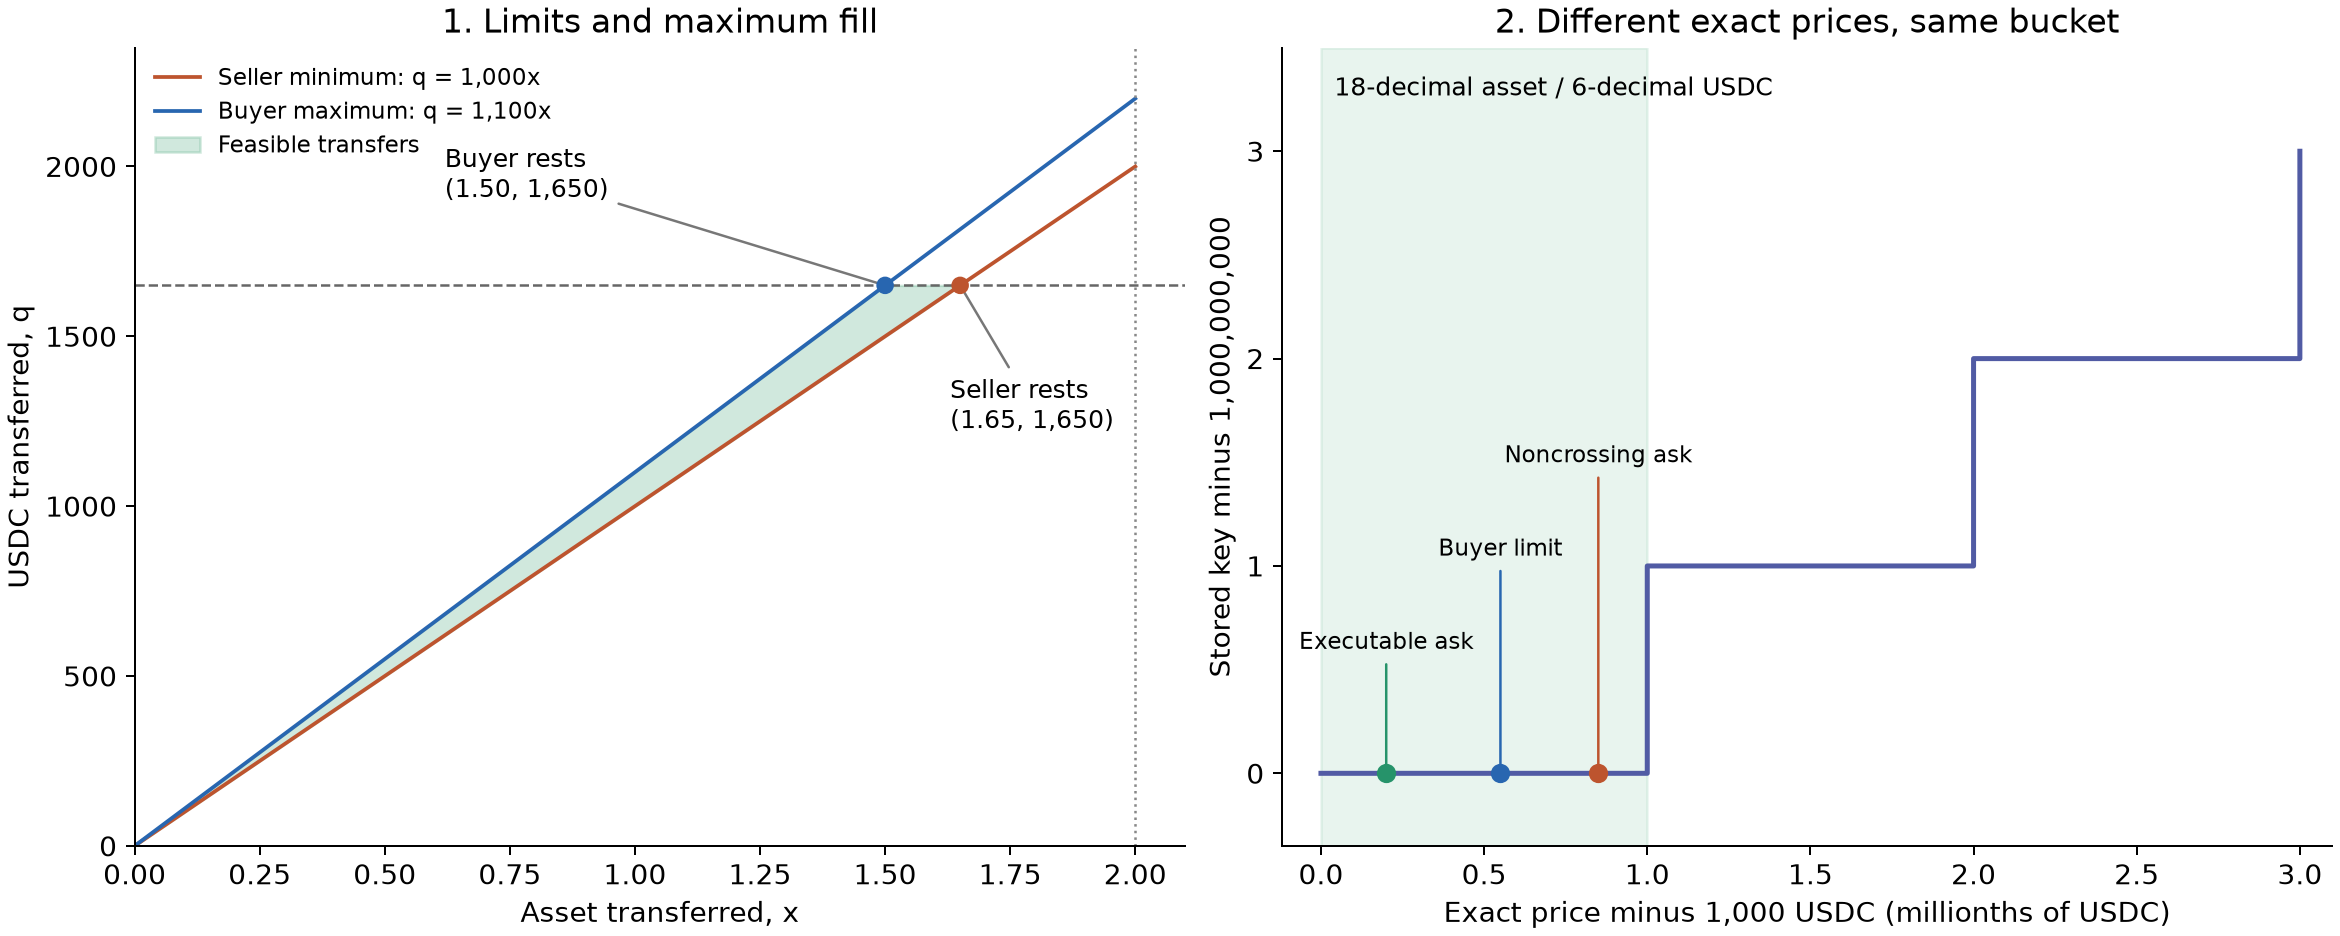
\includegraphics[width=\textwidth]{figures/matching-limits.png}
\caption{Left: feasible transfers and binding limits, in whole-token units.
Right: distinct exact prices within one price bucket.}
\end{figure}

\section{Priority among exactly eligible orders}

\subsection{Price buckets and priority}

Let $\sigma>0$ be a price scale and $K_{\max}$ the largest index key. The bucket of an exact
base-unit price $p$ is
\begin{equation}
 K(p)=\min\{K_{\max},\max\{1,\lfloor\sigma p\rfloor\}\}.
 \label{eq:bucket}
\end{equation}
This map is monotone. A bid bucket above an ask bucket therefore implies crossing; a bid
bucket below an ask bucket excludes it. Equal keys require the exact comparison
$Q_sA_b\le BS$. Index equality is not price equality.

If the asset has $d_a$ decimals and USDC has $d_u$ decimals, the human-unit price is
$P=p\,10^{d_a-d_u}$. An ordinary bucket has width
\begin{equation}
 \Delta=\frac{10^{d_a-d_u}}{\sigma}
 \quad\text{USDC per whole asset}.
\end{equation}
For $\sigma=10^{18}$, an 18-decimal asset, and six-decimal USDC, $\Delta=10^{-6}$.
For $K_{\max}>1$, bucket 1 covers $(0,2\Delta)$ and the top bucket covers
$[K_{\max}\Delta,\infty)$, before finite amount restrictions. The ordinary width bound
does not apply to these clamped buckets.

Within a bucket, order $i$ has priority $r_i=(f_i,-s_i)$, compared lexicographically:
a larger remaining bid $f_i$ ranks first, with earlier sequence $s_i$ breaking ties.
This is priority within a price group, rather than strict exact-price priority inside that
group. A bid affects rank only among orders compatible with the counterparty's limit.

Consider two asks in one bucket with $p_1\le p_b<p_2$, where the ask at $p_2$ has higher
priority. Inspecting only that ask misses the feasible trade at $p_1$. More generally,
inspecting only the first $L$ orders can miss a feasible order behind $L$ incompatible
ones. A finite inspection budget therefore requires an index of eligibility, not merely
a priority queue.

\subsection{Subtree summaries and selection}

Within each price bucket, arrange priority keys in a compressed binary tree. The right
subtree contains higher-priority keys. For every subtree $v$, maintain
\begin{equation}
 L(v)=\min_{i\in v}p_i\quad\text{for asks},\qquad
 U(v)=\max_{i\in v}p_i\quad\text{for bids}.
 \label{eq:summaries}
\end{equation}
An ask subtree contains an eligible order for a buyer at $p_b$ exactly when $L(v)\le p_b$;
a bid subtree contains one for a seller at $p_s$ exactly when $U(v)\ge p_s$.
Rational prices are compared by cross-products without rounding.

If the root is eligible, descend to the right child whenever its summary is eligible,
and otherwise to the left. The left child must then be eligible: the parent contains an
eligible order and its right child contains none. Every accepted right subtree outranks
the left subtree, so induction yields the highest-priority eligible leaf. No backtracking
or linear scan is required. In a compressed tree of $w$-bit keys, branch positions strictly
decrease along a path, giving at most $w$ branch decisions.

Each insertion, removal, repricing, or partial fill updates the affected subtree summaries
to preserve \eqref{eq:summaries}. Both searches and updates are bounded by the tree depth.

\subsection{Selecting a pair}

Selection is book-wide. An incoming order is first admitted to the book; the same rule then
selects pairs from the whole book, so a new order and any crossed backlog compete under one
priority order and share one bound on the number of pairs processed per call. Choose the highest bid bucket and
the lowest ask bucket. When their
keys are equal, let $\mathcal B$ and $\mathcal S$ be their orders and select
\begin{align}
 b^*&=\mathop{\mathrm{arg\,max}}_{b\in\mathcal B:\ p_b\ge\min_{s\in\mathcal S}p_s}r_b,\\
 s^*&=\mathop{\mathrm{arg\,max}}_{s\in\mathcal S:\ p_s\le p_{b^*}}r_s.
\end{align}
This maximizes $(r_b,r_s)$ lexicographically over feasible pairs in the boundary bucket:
buy priority first, then sell priority for the selected buy. When the best bid bucket is
strictly above the best ask bucket, their priority heads cross. Checking two crossing
heads directly gives the same result. An incompatible order remains open when skipped.

\begin{proposition}[Selection progress]
In a valid book containing a crossing pair, the selection rule finds a crossing pair,
assuming exact subtree summaries and unique priority ranks.
\end{proposition}
\begin{proof}
The highest bid key is at least the lowest ask key, by monotonicity of $K$.
If the inequality is strict, the priority heads cross. If the keys are equal, any crossing
pair must lie in those boundary buckets: a higher ask key or lower bid key cannot cross.
The minimum ask summary therefore identifies a nonempty set of feasible buys. The
priority search selects $b^*$ from that set, and a second search selects an ask crossing
$b^*$. Both searches terminate within the index depth bound.
\end{proof}


\section{Integer settlement and remaining orders}

The order created earlier in the selected pair is the maker and determines the reference
price. Creation order is fixed when an order is admitted: repricing and partial fills may
change an order's queue sequence, but not which of two orders was created first. When the
seller is earlier, settle
\begin{equation}
 x=\min\{S,\lfloor BS/Q_s\rfloor\},\qquad q=\lceil xQ_s/S\rceil.
 \label{eq:seller}
\end{equation}
When the buyer is earlier, settle
\begin{equation}
 q=\min\{B,\lfloor SB/A_b\rfloor\},\qquad x=\lceil qA_b/B\rceil.
 \label{eq:buyer}
\end{equation}
The ceiling protects the earlier order's minimum. The following result establishes that
the other order's minimum is also respected.

\begin{proposition}[Positive feasible settlement]
For positive integer order amounts satisfying \eqref{eq:cross}, either settlement rule
produces positive integers $x,q$ satisfying \eqref{eq:feasible}.
\end{proposition}
\begin{proof}
For \eqref{eq:seller}, if $x=S$, then $q=Q_s\le B$, and crossing gives
$xB=SB\ge Q_sA_b=qA_b$. Otherwise $x=\lfloor BS/Q_s\rfloor<S$.
Crossing implies $x\ge A_b\ge1$, while $q=\lceil xQ_s/S\rceil\le B$.
Hence $xB\ge A_bB\ge A_bq$. In both cases the ceiling gives $qS\ge xQ_s$.
For \eqref{eq:buyer}, if $q=B$, then $x=A_b\le S$ and crossing gives
$qS\ge xQ_s$. Otherwise $q=\lfloor SB/A_b\rfloor\ge Q_s\ge1$ and
$x=\lceil qA_b/B\rceil\le S$, so $qS\ge Q_sS\ge Q_sx$.
The ceiling gives $xB\ge qA_b$ in either case.
\end{proof}

For either side, write $I$ for its input before a fill, $O$ for its minimum output, and
$u$ for the input consumed. A surviving remainder has
\begin{equation}
 I'=I-u,\qquad O'=\left\lceil\frac{OI'}{I}\right\rceil.
 \label{eq:remainder}
\end{equation}
When $I'>0$, $O'/I'\ge O/I$: the remainder never asks for a worse exchange rate.
Price improvement on a completed fill does not reduce the remaining limit. Rounding can
change the exact ratio even when its bucket stays the same, so the eligibility summaries
must be refreshed after every partial fill.

A remainder below the market's minimum admitted notional closes and its unused input is
returned. For a buy, this notional is its remaining USDC input; for a sell, its remaining
minimum USDC output. A maker may cancel an open remainder or replace its minimum with a
new positive amount. Repricing assigns a fresh arrival sequence, as does a partial fill
that changes the price bucket. A partial fill otherwise retains its sequence; its remaining
bid determines fee priority. The arrival sequence governs queue priority only; the maker
role in a later match still follows creation order.

\section{Escrow, fees, and alternative counterparties}

Uniswap v4 provides a shared settlement layer and hook-based custom accounting, allowing
order settlement to coexist with pool liquidity~\cite{UniswapV4}. Async Swap uses this layer
to reserve assets and settle an exchange atomically. For each currency $c$, let $E_c$ denote
assets reserved for orders and let $I_{i,c}$ denote order $i$'s remaining input in that currency.
The order-escrow accounting condition is
\begin{equation}
 E_c=\sum_{i\in\mathcal O}I_{i,c}
       +\mathbf 1_{\{c=\mathrm{USDC}\}}\sum_{i\in\mathcal O}f_i,
 \label{eq:escrow}
\end{equation}
where $\mathcal O$ is the set of open orders and $f_i$ their remaining priority bids.
A transition reduces reserved balances only by the corresponding proceeds, refunds, or
settled fees. Each currency is conserved separately. Failed settlement leaves the exchange
uncommitted; amounts cannot be released twice. An owner or an explicitly authorized party
controls order changes and cancellation.

Reserved amounts are held as Uniswap v4 claims rather than token balances. A match pays
both sides, and refunds any remainder closed below the minimum, by moving these claims to
the recipients; no token transfer occurs during matching, so matching runs no token or
recipient code. A recipient redeems claims for the underlying tokens through a separate
redemption contract. A filler or pool-liquidity fill pays a token output directly, after
the order is closed; native-currency output is credited as claims.

Direct order matching has no additional exchange fee. If a fill consumes $u$ of input $I$,
the settled portion of a remaining priority bid $f$ is
\begin{equation}
 d=\left\lfloor\frac{fu}{I}\right\rfloor,\qquad f'=f-d.
\end{equation}
Any residual bid is settled when the order closes, including cancellation. Priority bids
are therefore non-refundable. Every settled bid goes to the protocol fee reserve; none
accrues to liquidity providers.

An unmatched remainder has two additional execution routes. It may trade against pool
liquidity if the entire remaining input can produce at least its minimum output after the
pool fee. Alternatively, an independent filler supplies that minimum output and receives
the remaining escrowed input. The latter route settles the full remainder, with the maker's
minimum $O$ defined net of the filler settlement fee:
\begin{equation}
 \Phi(O)=\left\lfloor\frac{3O}{997}\right\rfloor,\qquad
 \text{filler payment}=O+\Phi(O).
\end{equation}
The fee is approximately $0.3\%$ of the gross payment, subject to base-unit rounding.
A filler can impose a payment cap. Whether a fill is worthwhile depends on external prices,
fees, and execution costs; the maker's limit alone does not imply filler profit.

\section{Bounded work and parameter selection}

Let $w$ be the width of the binary index keys and $M$ the maximum number of pairs processed
in one matching call. Each pair requires a constant number of searches and updates, each
of depth at most $w$. The book's work is therefore $O(Mw)$, independent of the number of
ineligible orders in a bucket. With $w=128$, each traversal has at most 128 branches.
This bounds index work; a numerical transaction-cost bound also requires bounds on token
transfers and other settlement operations.

To relate throughput and cost, suppose a specified workload admits an affine cost envelope
$G(m)\le g_0+gm$, with fixed entry cost $g_0\ge0$ and per-pair bound $g>0$.
For budget $G_{\mathrm{budget}}\ge g_0$, the largest batch certified by this envelope is
\begin{equation}
 M^*=\min\left\{M_{\max},\left\lfloor\frac{G_{\mathrm{budget}}-g_0}{g}\right\rfloor\right\}.
 \label{eq:budget}
\end{equation}
It bounds permitted work, not the number of counterparties available. For the affine model,
total cost increases with $m$, while cost per pair satisfies
\begin{equation}
 \overline G(m)=g+\frac{g_0}{m},\qquad
 \frac{d\overline G}{dm}=-\frac{g_0}{m^2},\quad m>0.
\end{equation}
Smaller batches reduce total transaction cost; larger batches amortize entry cost. There
is no batch size that simultaneously minimizes total gas and maximizes matches without a
budget or another explicit tradeoff. A bound per call also does not bound the cost of a
transaction that composes several calls.

Price resolution controls grouping, not the validity of a trade. Making buckets narrower
cannot replace exact eligibility. Similarly, a minimum order size or bid floor can influence
the cost of occupying the book, but cannot create a crossing counterparty. The bid floor is parameterized by $f_{\min}(N)=\min\{f_{\mathrm{cap}},\lfloor\beta N\rfloor\}$, where $N$ is the
order's USDC notional. The choices $f_{\mathrm{cap}}=100000$ base units and $\beta=10^{-3}$
correspond to the smaller of $0.10$ USDC and $0.1\%$ of notional. These economic parameters
require calibration to order sizes and execution costs; the matching conditions do not
identify an economically optimal fee.

\section{Scope of the guarantees}

Exact limits and correct index summaries ensure that an incompatible priority head cannot
hide a feasible pair. They do not ensure an eventual fill for every order: compatible orders
may never arrive, higher-priority arrivals may continue, and execution requires someone to
submit a transaction. Priority bids rank orders inside the book; transaction inclusion and
ordering remain outside that ranking. Orders are public, so their limits and sizes reveal
trading intent.

USDC provides a common numeraire for comparing asset values. Equal USDC reference values do
not imply equal token quantities or equal net proceeds after fees and execution costs.
The model describes settlement within one market; a common numeraire alone does not provide
atomic settlement across chains.

\printbibliography
\end{document}
